\chapter{Conclusions and Future Work}\label{ch:conclusion}\addtocontents{lof}{\protect\contentsline{chapter}{\protect\numberline{\thechapter}Conclusion}{}{}}
\section{Conclusions}
In this thesis, a mock tricuspid valve was developed to improve the accuracy and functionality of right heart simulators. Through careful design and development, a model was created that accurately replicates the anatomical and biomechanical properties of the natural tricuspid valve and integrates effectively with existing simulation systems.

Challenges related to material compatibility and complex valve dynamics were addressed through advanced material testing and iterative design modifications. A prototype was produced, setting a new standard for realistic and functional heart valve simulators and potentially improving patient outcomes in cardiac care.

This work establishes a foundation for future research, suggesting further innovations in material technology and dynamic simulation capabilities. The anticipated integration of sophisticated computational models and exploration of new materials is expected to advance the capabilities of heart valve simulators significantly, bridging the gap between theoretical research and clinical application, and advancing biomedical engineering in cardiac care.

\newthought{In conclusion,} this study shows how the design process can be fraught with many more obstacles of many more varieties than expected. It resulted more in learnings of the iterative process of design and prototyping compared to test method development than expected.
% The study resulted in a manufacturing process that is consistent and effective in producing anatomically accurate valve models, developed over many different approaches with the strengths taken from each and weaknesses phased out. It also resulted in a test method that was able to effectively test the basic efficacy of the produced valves in a controlled environment and potential to very easily be adapted to introduce a variety tricuspid valve medical devices with simple fixturing and also account for variables like; pressure, flow rate, flow field, and regurgitant characteristics like orifice and volume, once integrated with the right heart simulator.
% The implications this type of testing could have on the development of \gls{TTVR} devices is significant. The ability to test the efficacy of these devices in a controlled environment can provide important data that can influence design choices and potentially mitigate against the risk of device failure in the clinical investigations.

\section{Future Research Directions}
Briefly touched on in the discussion were a few areas that further development in this project is very promising, continuing to decrease valve thickness will likely yield even more representative results and weaving chordal attachments into the leaflets will improve repeatability of fabrication while also aligning models more closely to that of \gls{CAD} designs for computational models.

% Pressure monitoring during test, 36\% glycerin for blood viscosity - rabbah
% In vitro micro ct scanning
\begin{figure}[H]
    \begin{fullwidth}
        \centering
        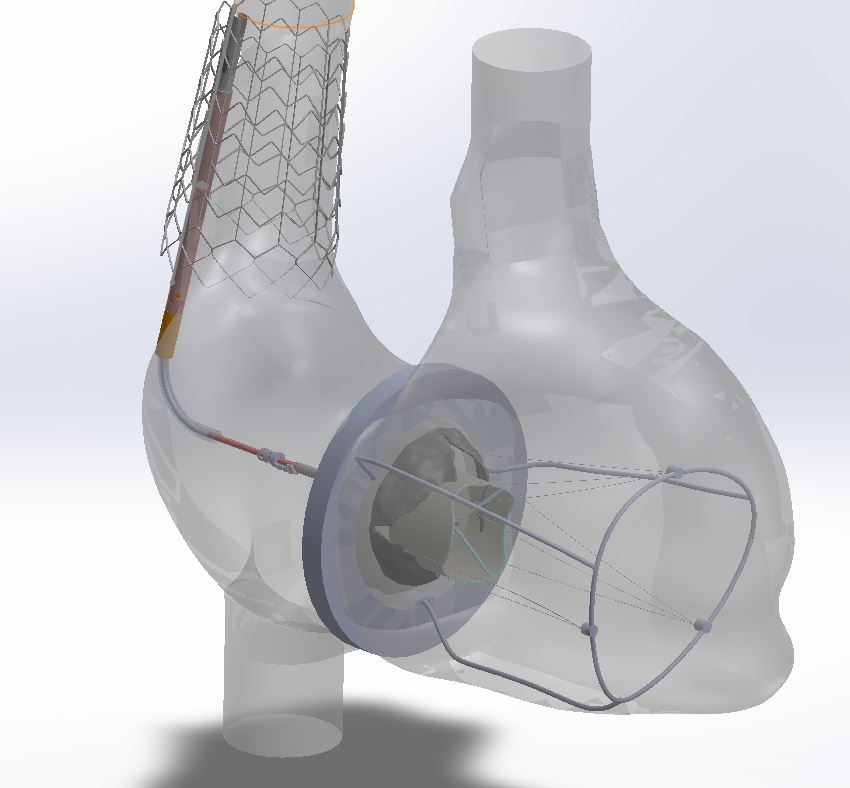
\includegraphics[width=0.8\textwidth]{figures/future}
        \caption{An assembly of the CroiValve DUO device in the right heart simulator}
        \label{fig:duo_assembly}
    \end{fullwidth}
\end{figure}
The next steps in this research will primarily be to fully integrate this valve into the right heart simulator. From there the rig be enhanced to involve \gls{TTVR} devices to characterize their efficacy on regurgitant valves. The main prospective device to integrate is the CroiValve DUO device which partially occludes the annulus of the valve reducing  regurgitant flow. While not reaching full fabrication due to time constrants, an assembly of what this would look like was created to illustrate how this would look. The models of the right heart simulator was used in designing the fixturing to them flush against the heart chamber for minimal flow disturbance.

Integration of the DUO device system could be carried out quite simply by implanting it aligning with the clinical procedure by anchoring the stent in the superior vena cava of the right heart simulator.

% At the moment the CroiValve team don't have the means to conduct work of this nature so the data collected in this study could be used to inform the design inputs of later interations.